

This chapter introduces the individual tests and what was included in each of them, in addition to 
the results collected from the tests.
The following results use both measurements, the conversion rate, and the click-through rate as previously introduced.
Furthermore, the conversion rates in the following tables are the conversion rate of the customers
that used the search application.
Also, the CTR shown in the first three tests is measured in the search result page from the subset of customers
that did not use any filters when they visited the page, and in \emph{Test 4}, the click-through rate included all
customers.
In the following descriptions, \emph{Variant A} is not referred to 
since it served as the baseline in all the concluded tests.


The results for the first three tests include the three different variants per test,
as each variant constructed the query differently.
\emph{Test 4} includes the measurements across different websites since the last test concluded included
the best parts from the previous three tests.
Furthermore, the fourth test was done in three different countries to see if the same solution could be applied
across the Nordic countries.

%% ==========================================================
%% TEST 1
%% ==========================================================

\emph{Test 1} included the first iteration of the ranking algorithm that boosted the products purely based
on the popularity rating.
In addition, the test included a query that was the first iteration of the one previously introduced in Figure \ref{fig:new-query}.
The query worked similarly and had the custom edge-N-gram analyzers with a wildcard character at the start and the end
of the search terms.
The query was not separately introduced in Section \ref{ss:methodsRanking} since the query was similar to the first query
from the introduced multiple queries setup.
In \emph{Test 1}, \emph{Variant B} included only the new query, \emph{Variant C} included only the new ranking function,
and \emph{Variant D} included both the new query and the new ranking function.

Figure \ref{fig:search_v1} shows that \emph{Test 1} increased the CTR of the top products when the new ranking function 
was utilized, in \emph{Variant C} and \emph{Variant D}.
However, the usage of the new ranking function decreased conversion rate, shown in Figure \ref{fig:search_v1}, most likely
due to the ranking algorithm not boosting the products that are in stock over the ones that are not.
While the conversion did not increase with the new ranking function, the effect of the new query can be seen with \emph{Variant B}.
Furthermore, the conversion rate slightly increases, and also the CTR of the top of the product list seems to be increased slightly.
The usage of the edge-N-gram analyzers in the new query for more meaningful token generation seemed to make the CTR increase
slightly. 


%% ==========================================================
\begin{figure}[p]
    \centering
    
    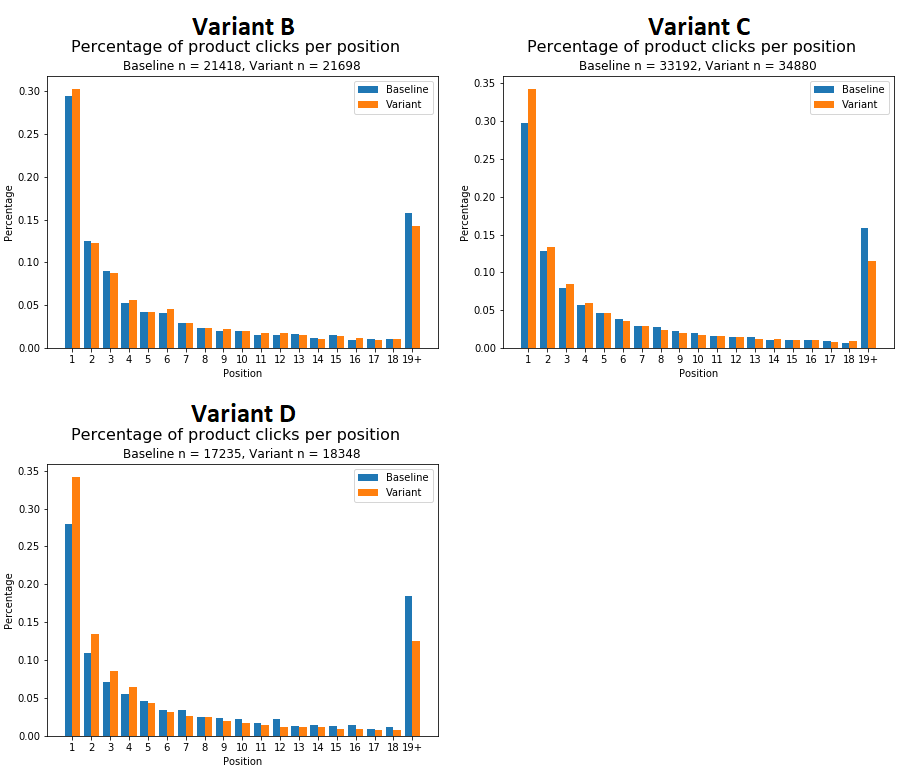
\includegraphics[width=\textwidth]{img/search_v1.png}

    %% ==========================================================
    \begin{tabular}{|c||c|c||c|c||c|c|}
    \hline
    \multicolumn{7}{|c|}{Test 1: Conversion rate from search} \\ \hline \hline
    & \multicolumn{2}{|c||}{Variant B} & \multicolumn{2}{|c||}{Variant C} & \multicolumn{2}{|c|}{Variant D} \\ \cline{2-7}
    & Baseline & Variant & Baseline & Variant & Baseline & Variant \\ \hline
    Sessions & 59 359 & 58 587 & 85 764 & 85 511 & 55 246 & 55 444 \\ \hline
    Conversion rate & 3,32\% & 3,43\% & 2,37\% & 2,19\% & 1,71\% & 1,52\% \\ \hline
    \end{tabular}

    \caption{Test 1: CTR and Conversion rates across variants.}
    \label{fig:search_v1}
\end{figure}

%% ==========================================================
%% TEST 2
%% ==========================================================


In \emph{Test 2}, both the ranking algorithm and the query were upgraded.
While the ranking algorithm in the previous test did not include the stock status of a product, a value
that was calculated was added to the index and used by the ranking algorithm.
Furthermore, \emph{Variant B} and \emph{Variant D} utilized the new ranking algorithm.
The previous query was updated to the one shown in Figure \ref{fig:new-query}, and it was
utilized by \emph{Variant C} and  \emph{Variant D}.

Figure \ref{fig:search_v2} shows, again, an increase when the ranking algorithm was utilized.
However, the multiple query setup did not seem to have an actual effect, although it seemed to perform
considerably better during the development.
The effect \emph{Test 2} had on conversion rate can be seen in Figure \ref{fig:search_v2}.
Furthermore, the conversion rate seems to be slightly increased in all variants.

The result did not meet the expectation set before the test, as the first test showed that conversion decrease as the
products might have been out of stock.
However, the expectation was that the conversion rate would be increased since the new ranking algorithm 
boosted the products in stock higher.
In addition, it seems that the usage of the analyzer in the specific fields is not optimal, as it seems to increase
the CTR, but not the conversion rate.


%% ==========================================================
\begin{figure}[p]
    \centering
    
    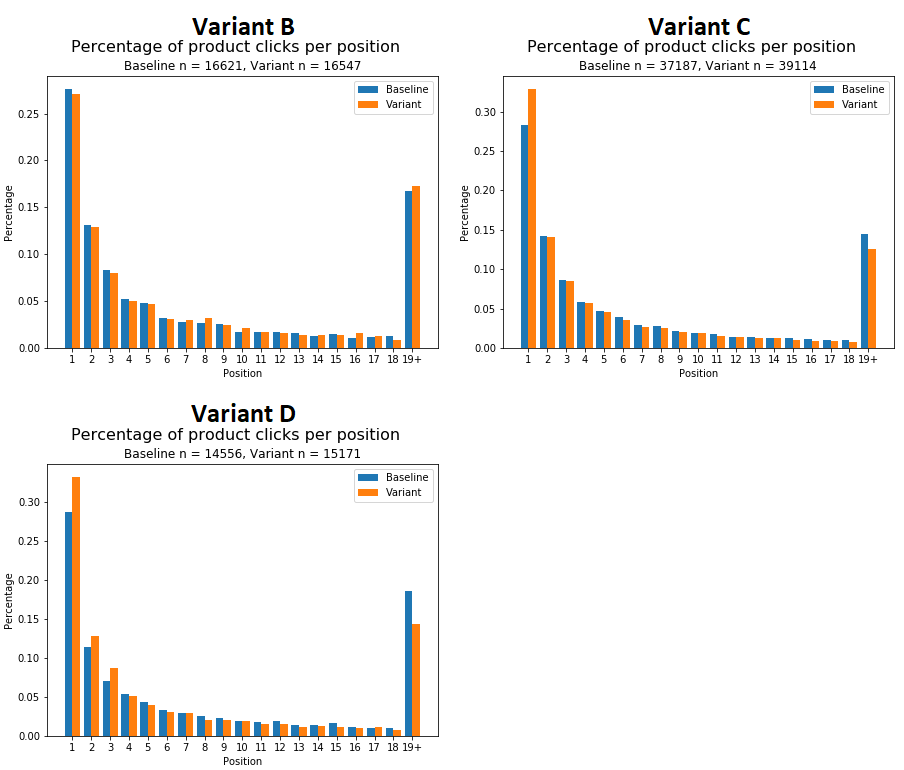
\includegraphics[width=\textwidth]{img/search_v2.png}

    %% ==========================================================
    \begin{tabular}{|c||c|c||c|c||c|c|}
    \hline
    \multicolumn{7}{|c|}{Test 2: Conversion rate from search} \\ \hline \hline
    & \multicolumn{2}{|c||}{Variant B} & \multicolumn{2}{|c||}{Variant C} & \multicolumn{2}{|c|}{Variant D} \\ \cline{2-7}
    & Baseline & Variant & Baseline & Variant & Baseline & Variant \\ \hline
    Sessions & 47 884 & 47 866 & 89 820 & 88 990 & 45 472 & 46 414 \\ \hline
    Conversion rate & 3,04\% & 3,20\% & 4,84\% & 4,95\% & 1,45\% & 1,46\% \\ \hline
    \end{tabular}

    \caption{Test 2: CTR and Conversion rates across variants.}
    \label{fig:search_v2}
\end{figure}


%% ==========================================================
%% TEST 3
%% ==========================================================


While the previous two tests included three different variables, \emph{Test 3} only included two.
Both \emph{Variant C} and \emph{Variant D} included the same ranking function and multiple queries as 
\emph{Test 2}.
However, instead of using \emph{MUST} clauses with multiple search terms, \emph{SHOULD} clause was used.
Furthermore, this meant that by searching with multiple search terms, all matches that matched any of 
the search terms were included, but the results that matched several terms were boosted accordingly higher.

Figure \ref{fig:search_v3} shows that the CTR of the search result list on the subset of customers who did not 
use the product filters after searching did not change significantly.
Still, the conversion rate was increased in both different variants, as shown in Figure \ref{fig:search_v3}.
The described behavior did not meet expectations, as the same ranking algorithm was utilized as in \emph{Test 2},
the expected result was that the CTR would have been at a similar level as well.


%% ==========================================================
\begin{figure}[p]
    \centering
    
    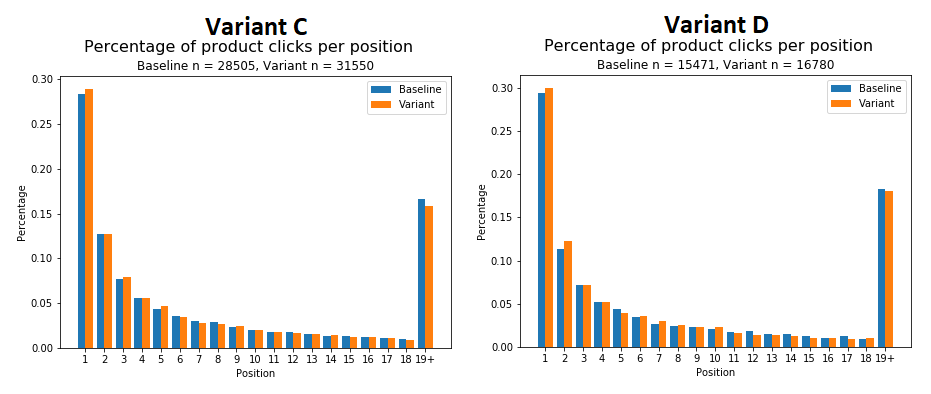
\includegraphics[width=\textwidth]{img/search_v3.png}

    %% ==========================================================
    \begin{tabular}{|c||c|c||c|c|}
    \hline
    \multicolumn{5}{|c|}{Test 3: Conversion rate from search} \\ \hline \hline
    & \multicolumn{2}{|c||}{Variant C} & \multicolumn{2}{|c|}{Variant D} \\ \cline{2-5}
    & Baseline & Variant & Baseline & Variant \\ \hline
    Sessions & 79 894 & 81 279 & 52 575 & 51 814 \\ \hline
    Conversion rate & 2,27\% & 2,35\% & 1,37\% & 1,44\% \\ \hline
    \end{tabular}
    \caption{Test 3: CTR and Conversion rates across variants.}
    
    \label{fig:search_v3}
\end{figure}



%% ==========================================================
%% TEST 4
%% ==========================================================

The fourth and final test was concluded based on the previous tests, introduced above.
In addition to the testing setup used in \emph{Test 2}, this test included a functionality that, while 
querying the results, queried a suggested search term at the same time.
Then, if the query did not match any products, the query would be rerun with the suggested word.
Furthermore, meaning that, for instance, if the customer misspelled a word and it resulted in zero results,
the suggested word would be searched with, and results with the correct term could be returned.


Furthermore, this functionality was designed to be similar to fuzzy search and was easier to implement,
due to the time limitations, as using the fuzzy search.
For the future development, the fuzzy search is most likely investigated properly, as fuzzy search does not 
work with wildcard searches, which were utilized by the queries, it could not be implemented for this thesis.

\emph{Test 4} the three variants again, but in this setup, all the variants utilized the same features.
In this test, the three variants mean three different websites in three different countries.
Furthermore, since the organization has multiple websites across the Nordic countries, it was crucial
to see if the solution proposed by this thesis performed well in all of the countries.


The results, in Table \ref{tab:search_v4_ctr}, show a remarkable increase in the CTR of the search result list.
Therefore, indicating that the relevancy of the search result was increased in \emph{Test 4}, at least when
measured with CTR.
However, the conversion rate was not increased by \emph{Test 4} that much, and in \emph{Variant D} even decreased.
While the solution in \emph{Test 4} seemed to satisfy the needs of the customers, at least better, the solution did
not seem to capture the needs of the organization, as the number of sales was not affected that significantly.

%% ==========================================================
\begin{table}[p]
    \centering
    
    \begin{tabular}{|c||c|c||c|c||c|c|}
    \hline
    \multicolumn{7}{|c|}{Test 4: CTR based on the product position} \\ \hline \hline
    \multirow{ 2}{4em}{List position} & \multicolumn{2}{|c||}{Variant B} & \multicolumn{2}{|c||}{Variant C} & \multicolumn{2}{|c|}{Variant D} \\ \cline{2-7}
    & Baseline & Variant & Baseline & Variant & Baseline & Variant \\ \hline
    1 & 21,99\% & 28,59\% & 19,92\% & 25,19\% & 21,98\% & 27,11\% \\ \hline
    2 & 14,32\% & 16,65\% & 12,71\% & 16,90\% & 12,38\% & 16,42\% \\ \hline
    3 & 11,28\% & 12,29\% & 10,14\% & 12,39\% & 10,58\% & 12,06\% \\ \hline
    4 & 8,15\% & 9,10\% & 8,55\% & 9,77\% & 8,14\% & 9,31\% \\ \hline
    5 & 6,92\% & 8,14\% & 7,51\% & 8,91\% & 6,74\% & 7,93\% \\ \hline
    6 & 6,43\% & 7,37\% & 6,29\% & 7,86\% & 6,19\% & 6,88\% \\ \hline
    7 & 6,46\% & 6,74\% & 5,95\% & 7,19\% & 6,01\% & 6,25\% \\ \hline
    8 & 6,05\% & 6,33\% & 5,87\% & 7,12\% & 5,59\% & 5,87\% \\ \hline
    9 & 5,93\% & 6,28\% & 5,78\% & 6,75\% & 5,70\% & 5,37\% \\ \hline
    10 & 6,19\% & 5,94\% & 5,69\% & 6,68\% & 4,80\% & 5,44\% \\ \hline
    \end{tabular}
    \caption{Test 4: CTR in the different websites.}
    \label{tab:search_v4_ctr}
    
    %% ==========================================================
    \begin{tabular}{|c||c|c||c|c||c|c|}
    \hline
    \multicolumn{7}{|c|}{Test 4: Conversion rate from search} \\ \hline \hline
    & \multicolumn{2}{|c||}{Variant B} & \multicolumn{2}{|c||}{Variant C} & \multicolumn{2}{|c|}{Variant D} \\ \cline{2-7}
    & Baseline & Variant & Baseline & Variant & Baseline & Variant \\ \hline
    Sessions & 119 609 & 119 535 & 189 661 & 192 392 & 105 572 & 108 762 \\ \hline
    Conversion rate & 3,89\% & 3,95\% & 2,78\% & 2,96\% & 2,47\% & 2,41\% \\ \hline
    \end{tabular}
    \caption{Test 4: Conversion rates in the different websites.}
    \label{tab:search_v4}
\end{table}


This chapter introduced the four different tests that were concluded for this thesis.
Each test had separate variants, which were measured from different websites in different countries.
In summary, the conclude test showed an increase in the click-through rate of the search product lists. 
However, the primary measurement, the conversion rate, was not significantly affected by the concluded tests.
The following chapter includes the conclusions that could be drawn from the results, in addition to including
subjects for future development.








